%!TEX root = Slic3r-Manual.tex

\section{Assistant de Configuration}
\label{sec:configuration_wizard}
\index{Assistant de Configuration}
\index{Configuration Wizard}

Slic3r a deux fonctions pour aider les nouveaux venus: l'assistant de configuration, et le mode simple.

Parfois, il est bon d'avoir un coup de main lors du d\'emarrage d'un nouveau logiciel. L'assistant de configuration pose une s\'erie de questions et cr\'ee une configuration de d\'emarrage pour Slic3r.

\begin{figure}[H]
\centering
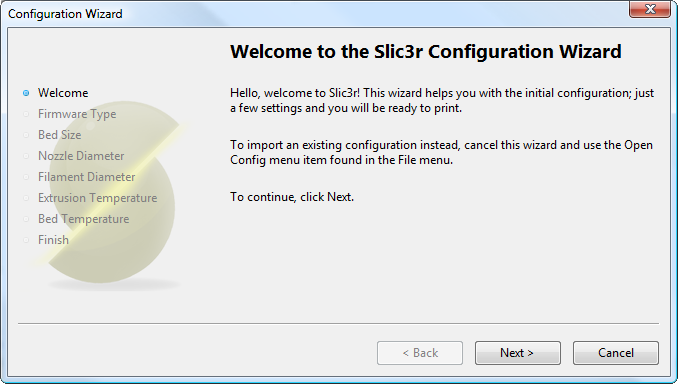
\includegraphics[keepaspectratio=true,width=\textwidth]{configuration_wizard/configuration_wizard_welcome.png}
\caption{Assistant de Configuration: \'Ecran de bienvenue}
\label{fig:configuration_wizard_welcome_screen}
\end{figure}

\newpage
\subsection{1. Type de Micrologiciel}
\label{sub:1_firmware_type}
\index{Printer Settings!Firmware!G-code flavour}
\index{Param\`etres de l'Imprimante!Micrologiciel!Variante du G-code}

Le G-code produit par Slic3r est adapt\'e \`a certains types de micrologiciel. La premi\`ere \'etape, demande le micrologiciel utilis\'e pour l'imprimante. Cela a d\^u \^etre sp\'ecifi\'e lorsque l'imprimante a \'et\'e construite ou configur\'ee. En cas de doute contactez le fournisseur.
\begin{figure}[H]
\centering
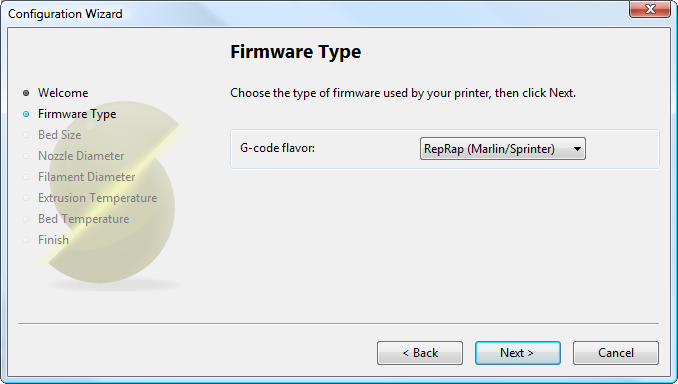
\includegraphics[keepaspectratio=true,width=\textwidth]{configuration_wizard/configuration_wizard_firmware_type.png}
\caption{Assistant de Configuration: Type de Micrologiciel}
\label{fig:configuration_wizard_firmware_type}
\end{figure}

\newpage
\subsection{2. Taille du Lit}
\label{sub:2_bed_size}
\index{Printer Settings!Size and coordinates!Bed size}
\index{Param\`etres de l'Imprimante!Taille et coordonn\'ees!Taille du Lit}

Ce param\`etre d\'efinit la distance maximale que l'extrudeuse peut parcourir le long de l'axe X et Y. Si les dimensions ne sont pas disponibles, elles peuvent \^etre facilement mesur\'ees.

N'oubliez pas de mesurer \`a partir du coin inf\'erieur gauche o\`u la buse d'extrusion repose quand elle est en position de repos jusqu'a la distance maximale que la buse peut ateindre pour chaque direction. Prenez en compte que le chariot de X peut toucher le cadre avant la buse atteigne sa limite, cela d\'ependra de la marque et du mod\`ele de l'imprimante.

Pensez \'egalement \`a v\'erifier les param\`etres de but\'ee du micrologiciel, qui peuvent limiter les d\'eplacement X / Y.

\begin{figure}[H]
\centering
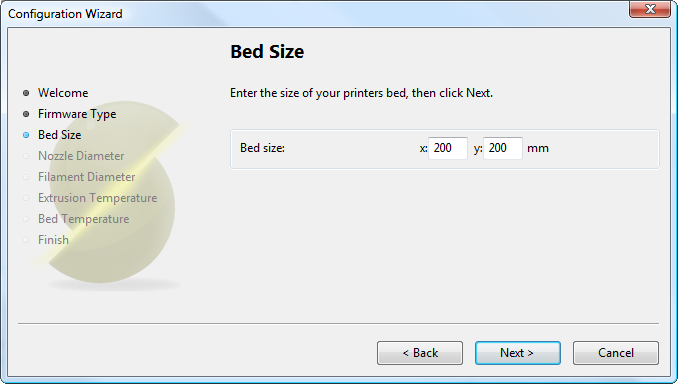
\includegraphics[keepaspectratio=true,width=\textwidth]{configuration_wizard/configuration_wizard_bed_size.png}
\caption{Assistant de Configuration: Taille du Lit}
\label{fig:configuration_wizard_bed_size}
\end{figure}

\newpage
\subsection{3. Diam\`etre de la buse}
\label{sub:3_nozzle_diameter}
\index{Printer Settings!Extruder!Nozzle diameter}
\index{Param\`etres de l'Imprimante!Extrudeuse!Diam\`etre de la buse}
Le diam\`etre de la buse est g\'en\'eralement clairement affich\'e soit dans la description de la t\^ete chauffante, ou dans la documentation associ\'ee, lorsque la t\^ete chauffante est achet\'e. Les valeurs courantes sont 0,5 mm et 0,35 mm.

Si la buse est faite maison, ou provient d'une source sans informations du diam\`etre, alors mesurez soigneusement l'ouverture aussi pr\'ecis\'ement que possible. Une fa\c{c}on de d\'eterminer la taille de la buse est d'extruder tr\`es lentement (1mm / s) un peu de filament \`a l'air libre, et de mesurer l'\'epaisseur de l'extrusion\footnote{\url{http://forums.reprap.org/read.php?1,113374,113953}}.  
Ceci a l'avantage de prendre en compte le gonflement \`a la fili\`ere, et par cons\'equent pourrait \^etre une chose utile \`a faire, m\^eme si le diam\`etre est connu.

\begin{figure}[H]
\centering
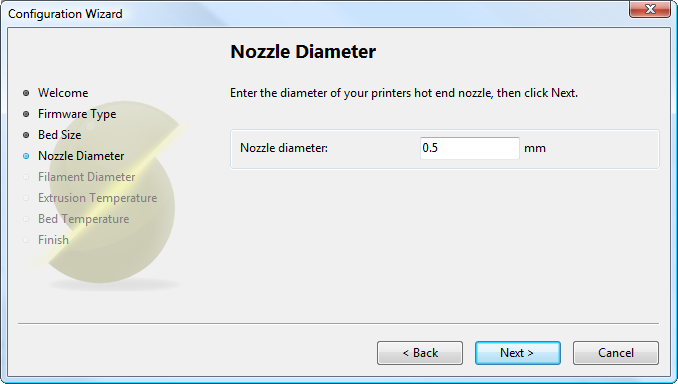
\includegraphics[keepaspectratio=true,width=\textwidth]{configuration_wizard/configuration_wizard_nozzle_diameter.png}
\caption{Assistant de Configuration: Diam\`etre de la buse}
\label{fig:configuration_wizard_nozzle_diameter}
\end{figure}

\newpage
\subsection{4. Diam\`etre du Filament}
\label{sub:4_filament_diameter}
\index{Filament Settings!Filament!Diameter}
\index{Param\`etres du Filament!Filament!Diam\`etre}
Pour que Slic3r produise des r\'esultats pr\'ecis, il doit conna\^itre aussi pr\'ecis\'ement que possible la quantit\'e de mati\`ere qui est pouss\'e \`a travers l'extrudeuse. Il est donc essentiel de lui donner la valeur la plus pr\'ecise possible pour le diam\`etre du filament.

Bien que le filament utilis\'e dans les imprimantes FDM soit vendu pour un diam\`etre de 3 mm ou 1,75 mm ce n'est qu'une indication . Le diam\`etre peut varier entre les fabricants et m\^eme entre les lots. Par cons\'equent, il est fortement recommand\'e de prendre des mesures multiples de long du filament et d'utiliser la moyenne. Par exemple, les mesures de 2.89, 2.88, 2.90 et 2.91 donneraient une moyenne de 2,895, \`a utiliser ici.

\begin{figure}[H]
\centering
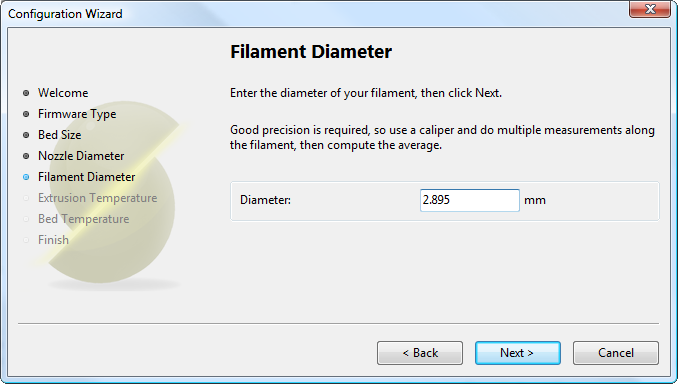
\includegraphics[keepaspectratio=true,width=\textwidth]{configuration_wizard/configuration_wizard_filament_diameter.png}
\caption{Assistant de Configuration: Diam\`etre du Filament}
\label{fig:configuration_wizard_filament_diameter}
\end{figure}

\newpage
\subsection{5. Temp\'erature d'Extrusion}
\label{sub:5_extrusion_temperature}
\index{Filament Settings!Temperature!Extruder}
\index{Param\`etres du Filament!Temperature!Extrudeuse}
La temp\'erature d'extrusion d\'epend de la mati\`ere, celle-ci peut fonctionner sur une large plage. Le fournisseur doit fournir des informations sur les temp\'eratures appropri\'es. Une r\`egle tr\`es g\'en\'erale est que la temp\'erature pour le PLA est comprise entre 160 ° C et 230 ° C, et que la temp\'erature pour l'ABS se situe entre 215 ° C et 250 ° C. Les mat\'eriaux plus exotiques auront une gamme diff\'erente.

C'est un param\`etre que vous aurez envie de peaufiner quand vous commencerez \`a produire des impressions. La temp\'erature optimale peut varier, m\^eme entre les couleurs de la m\^eme mati\`ere. Un autre facteur qui peut affecter la temp\'erature choisie, est la vitesse d'extrusion, g\'en\'eralement plus la vitesse est \'elev\'ee, plus la temp\'erature est \'elev\'ee.

Remarque: On peut choisir de r\'eguler la temp\'erature de l'extrudeuse manuellement \`a partir du contr\^oleur d'imprimante. Dans ce cas, la temp\'erature peut \^etre r\'egl\'ee \`a z\'ero.

\begin{figure}[H]
\centering
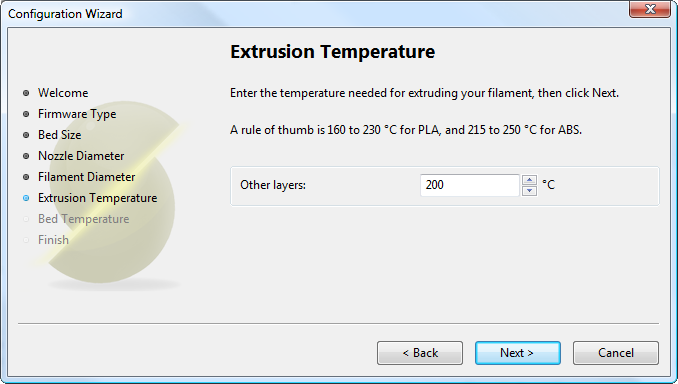
\includegraphics[keepaspectratio=true,width=\textwidth]{configuration_wizard/configuration_wizard_extrusion_temperature.png}
\caption{Assistant de Configuration: Temp\'erature d'Extrusion}
\label{fig:configuration_wizard_extrusion_temperature}
\end{figure}

\newpage
\subsection{6. Temperature du Lit}
\label{sub:6_bed_temperature}
\index{Filament Settings!Temperature!Bed}
\index{Param\`etres du Filament!Temperature!Lit}
Si l'imprimante dispose d'un lit chauff\'e ce param\`etre peut \^etre pr\'ecis\'e. Comme la temp\'erature de l'extrudeuse, la valeur d\'epend de la mati\`ere utilis\'ee. Une r\`egle de base est que PLA n\'ecessite ~ 60 ° C et ABS n\'ecessite ~ 110 ° C.

Remarque: On peut choisir de contr\^oler la temp\'erature du lit manuellement \`a partir du contr\^oleur d'imprimante. Dans ce cas, la temp\'erature peut \^etre r\'egl\'ee \`a z\'ero.

\begin{figure}[H]
\centering
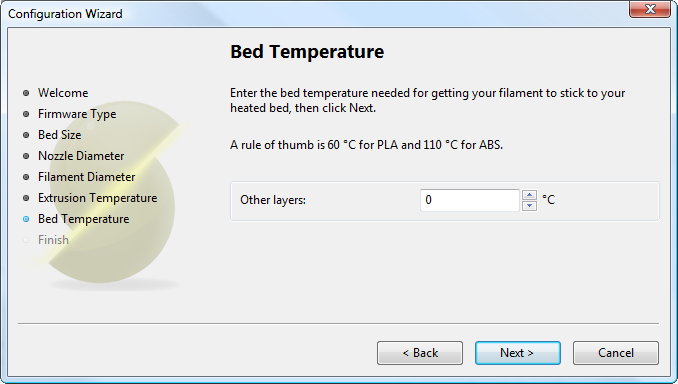
\includegraphics[keepaspectratio=true,width=\textwidth]{configuration_wizard/configuration_wizard_bed_temperature.png}
\caption{Assistant de Configuration: Temperature du Lit}
\label{fig:configuration_wizard_bed_temperature}
\end{figure}

\newpage

A ce stade, l'assistant est termin\'e et la configuration de base est d\'efinie.

\begin{figure}[H]
\centering
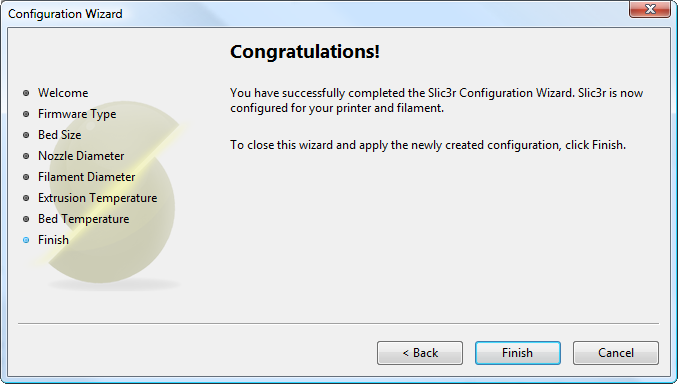
\includegraphics[keepaspectratio=true,width=\textwidth]{configuration_wizard/configuration_wizard_end.png}
\caption{Assistant de Configuration: Fin}
\label{fig:configuration_wizard_end}
\end{figure}

